\section{Phase II Step 1: C1 Stability Analysis}
\label{sec:phase2_c1_stability}

Month 3 starts with the most empirical comparison criterion: stability. The purpose of this step is to
measure how much each candidate signal changes across release windows and whether developer rankings remain
similar from one window to the next. This step does not select the PoC metric. It produces the first evidence
layer used later together with interpretability, gaming resistance, long-term suitability, and smart-contract
feasibility.

\subsection{Analysis inputs and generated artifacts}
\label{sec:c1_inputs_outputs}

The C1 script reads only the centralized Phase I \texttt{\_all} evidence. It writes derived Phase II artifacts
under \path{Data,Outputs,Logs,Scripts/Phase 2/}, keeping comparative-analysis outputs separate from the frozen
dataset and extraction layer.

\begin{table}[H]
\centering
\scriptsize
\renewcommand{\arraystretch}{1.08}
\begin{tabularx}{\textwidth}{>{\raggedright\arraybackslash}p{5.0cm}rX}
\toprule
\textbf{Artifact} & \textbf{Rows} & \textbf{Role} \\
\midrule
\path{out/c1_metric_window_values_all.csv} & 350 & Long-format window-level values for five stability signals across 70 windows. \\
\path{out/c1_metric_stability_by_project_all.csv} & 50 & Per-project volatility statistics for each stability signal. \\
\path{out/c1_metric_stability_overall_all.csv} & 5 & Cross-project summary of window-level volatility. \\
\path{out/c1_rank_input_values_all.csv} & 3189 & Developer-level values used for adjacent-window rank comparison. \\
\path{out/c1_rank_stability_pairs_all.csv} & 180 & Adjacent-window rank correlations for M2, M3, and M4 developer-level signals. \\
\path{out/c1_rank_stability_by_project_all.csv} & 30 & Per-project rank-stability summaries. \\
\path{out/c1_rank_stability_overall_all.csv} & 3 & Cross-project rank-stability summary. \\
\path{logs/c1_stability_20260508.log} & 1 & Execution log for the C1 stability run. \\
\bottomrule
\end{tabularx}
\caption{Phase II C1 stability artifacts. Paths are relative to the Phase II analysis directory.}
\label{tab:c1_artifacts}
\end{table}

\subsection{Method}
\label{sec:c1_method}

For window-level stability, five signals are compared:
\begin{itemize}[leftmargin=*]
  \item M1 endpoint KLOC, using the code-line count at each window's target tag;
  \item M2 churn per KLOC-day, using size- and duration-normalized churn;
  \item M3 commits per day, using duration-normalized activity cadence;
  \item M4 churn Gini, using contributor concentration in churn;
  \item M4 top-1 churn share, using the largest contributor's churn share.
\end{itemize}

For each project and signal, the script computes the coefficient of variation and adjacent-window relative
change. The same statistics are computed twice: once on all windows, and once on the robust subset that excludes
windows marked \texttt{sensitivity\_only}. For developer-level rank stability, the script compares adjacent
windows using Spearman rank correlation among developers who appear in both windows. Rank stability is computed
for M2 developer churn/day, M3 developer commits/day, and M4 developer churn share.

\subsection{Window-level stability results}
\label{sec:c1_window_results}

\begin{table}[H]
\centering
\scriptsize
\renewcommand{\arraystretch}{1.08}
\begin{tabular}{p{3.9cm}rrrr}
\toprule
\textbf{Signal} & \textbf{Median CV} & \textbf{Primary CV} & \textbf{Primary adjacent change} & \textbf{Primary high-vol. projects} \\
\midrule
M1 endpoint KLOC & 0.013 & 0.014 & 0.009 & 0 \\
M2 churn/KLOC/day & 1.208 & 0.890 & 0.706 & 6 \\
M3 commits/day & 0.876 & 0.608 & 0.644 & 4 \\
M4 churn Gini & 0.424 & 0.329 & 0.337 & 2 \\
M4 top-1 churn share & 0.289 & 0.236 & 0.208 & 1 \\
\bottomrule
\end{tabular}
\caption{C1 window-level volatility summary. CV is the coefficient of variation across project windows; ``primary'' excludes short windows marked \texttt{sensitivity\_only}.}
\label{tab:c1_window_stability_summary}
\end{table}

The first result is clear: M1 is stable because project size changes slowly between adjacent stable releases.
That stability makes it a useful context and normalization signal, but it does not directly measure developer
contribution quality or reputation. M2 and M3 are much more dynamic. Churn is especially volatile, which is
expected because release content can vary sharply even inside the same project. M4 concentration signals are
more stable than raw activity measures, with top-1 churn share showing the lowest volatility among behavior-oriented
signals in this pass.

\begin{figure}[H]
\centering
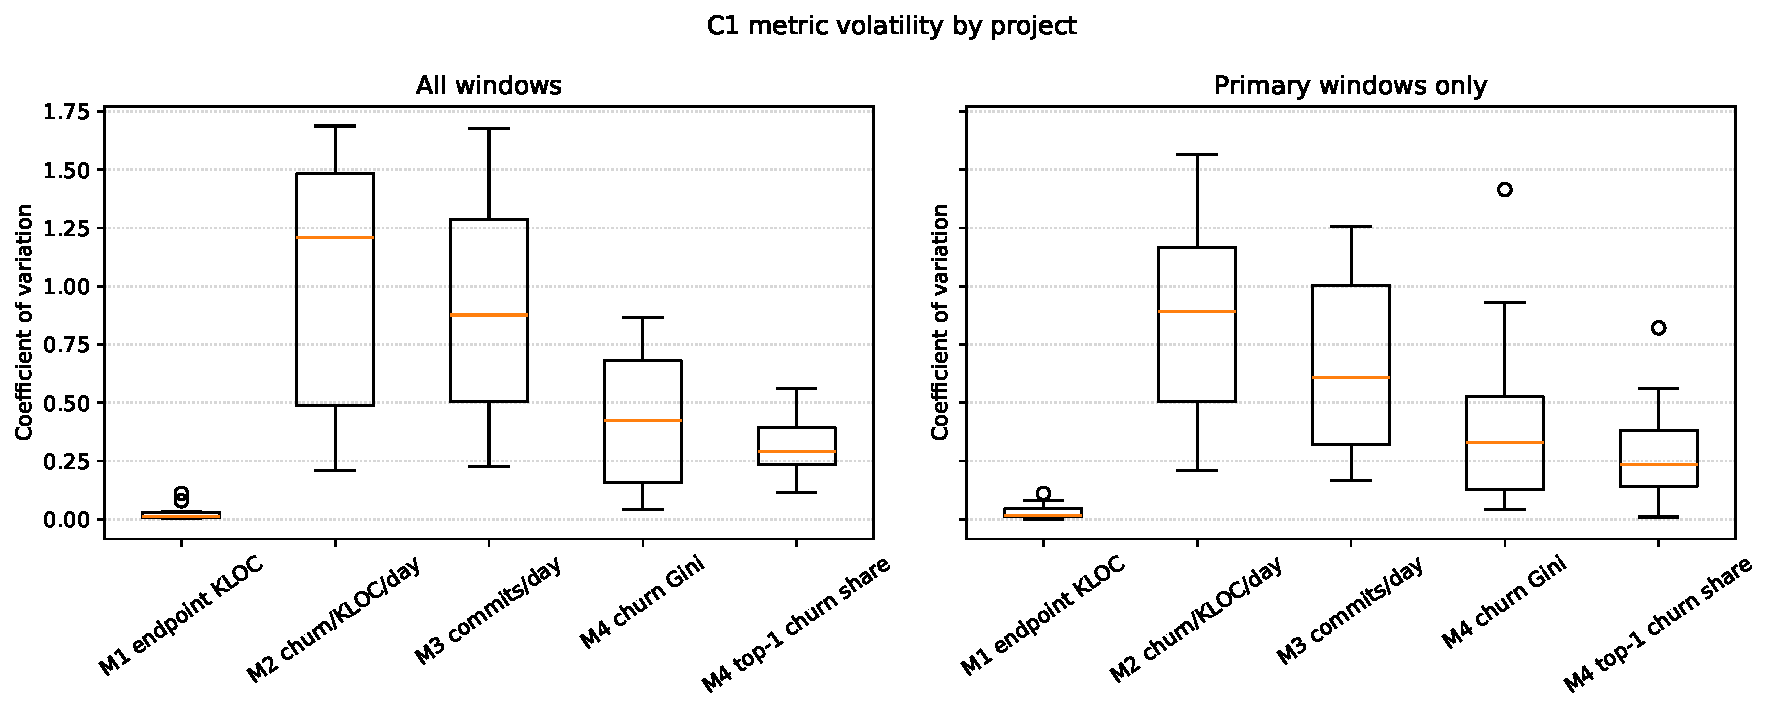
\includegraphics[width=\textwidth]{figures/month3_c1/c1_volatility_by_metric.pdf}
\caption{Distribution of per-project coefficient of variation for each C1 window-level signal.}
\label{fig:c1_volatility_by_metric}
\end{figure}

\begin{figure}[H]
\centering
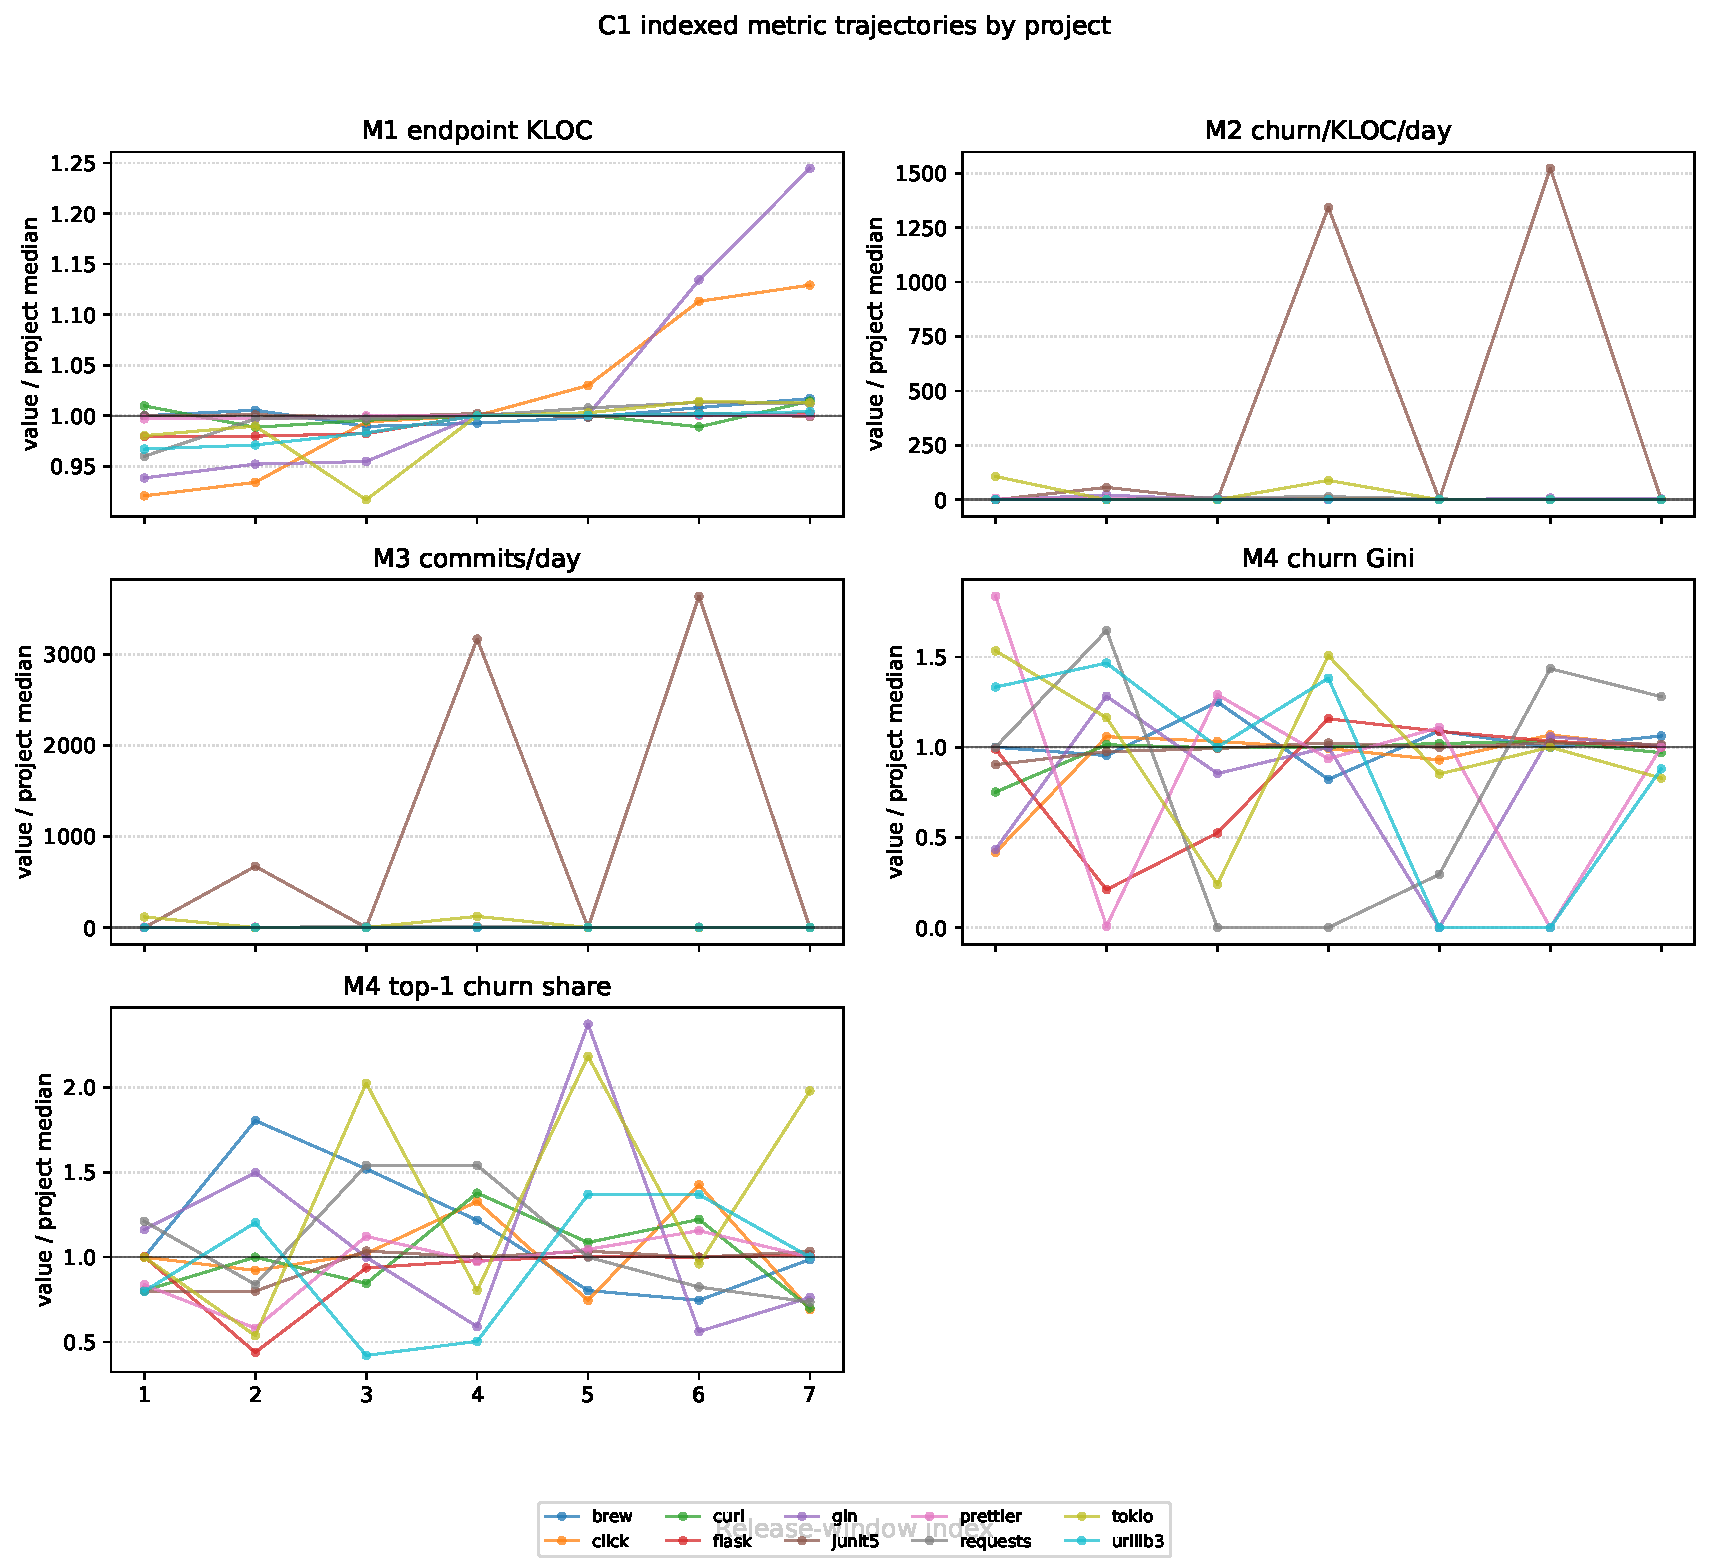
\includegraphics[height=0.72\textheight,width=\textwidth,keepaspectratio]{figures/month3_c1/c1_indexed_metric_trends.pdf}
\caption{Indexed C1 signal trajectories by project. Each line is scaled by that project's median value for the signal.}
\label{fig:c1_indexed_metric_trends}
\end{figure}

\subsection{Developer-rank stability results}
\label{sec:c1_rank_results}

\begin{table}[H]
\centering
\scriptsize
\renewcommand{\arraystretch}{1.08}
\begin{tabular}{p{3.8cm}rrrr}
\toprule
\textbf{Developer-level signal} & \textbf{Median $\rho$} & \textbf{Primary $\rho$} & \textbf{Common share} & \textbf{Valid pairs} \\
\midrule
M2 developer churn/day & 0.668 & 0.608 & 0.172 & 36/60 \\
M3 developer commits/day & 0.858 & 0.836 & 0.172 & 33/60 \\
M4 developer churn share & 0.668 & 0.608 & 0.172 & 36/60 \\
\bottomrule
\end{tabular}
\caption{C1 developer-rank stability summary across adjacent windows. Correlations use only developers appearing in both adjacent windows.}
\label{tab:c1_rank_stability_summary}
\end{table}

The rank-stability result should be read together with the common-developer share. The median overlap between
adjacent windows is only 0.172, so many adjacent windows involve a partially different contributor set. Among
developers who do recur, M3 commit cadence has the strongest rank continuity. M2 churn/day and M4 churn share
produce the same rank-stability values because churn share is a within-window normalization of churn; it changes
the unit and interpretation, but not the developer ordering inside the same window.

\begin{figure}[H]
\centering
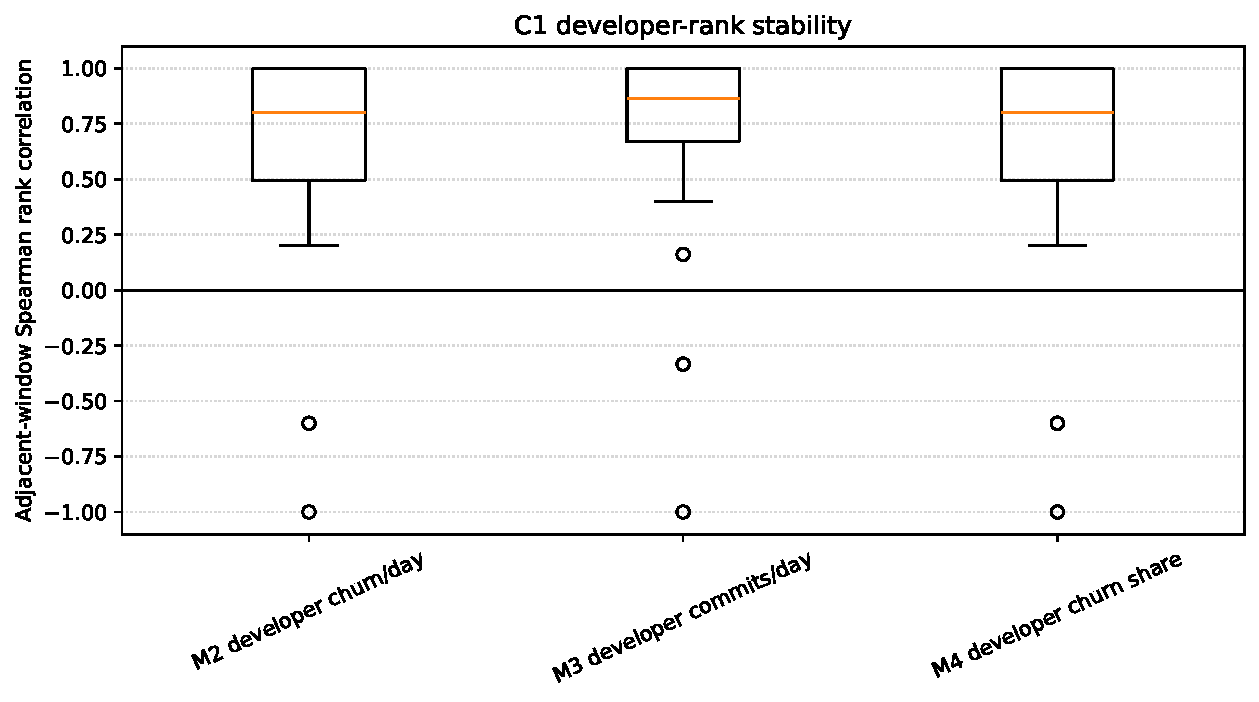
\includegraphics[width=0.82\textwidth]{figures/month3_c1/c1_rank_stability_by_metric.pdf}
\caption{Adjacent-window developer-rank stability for M2, M3, and M4 developer-level signals.}
\label{fig:c1_rank_stability}
\end{figure}

\subsection{C1 interpretation for the decision process}
\label{sec:c1_interpretation}

The C1 evidence does not select a final PoC metric, but it narrows the interpretation of the candidates:
\begin{itemize}[leftmargin=*]
  \item M1 is empirically stable but mainly useful as context and normalization support.
  \item M2 is informative about release effort but too volatile to use alone without safeguards.
  \item M3 has better developer-rank continuity than M2, but still depends on release cadence and contributor overlap.
  \item M4 concentration signals are comparatively stable and remain promising for reputation interpretation, but they require careful gaming-resistance analysis.
\end{itemize}

The next section evaluates C2 interpretability using the same candidate set and the C1 findings.
After C2, C3 gaming resistance and C4 long-term suitability can be scored before applying the smart-contract feasibility rubric.
